\section{StreamNet main algorithm}
\subsection{Based on the centrality (katz centrality) to COO starting point selection algorithm}
At this stage of the DAG, when selecting the tip, it will not start from the creation transaction, but will simply start with a coordinator as the starting point. This will lead to a centralization problem. So the first question we considered when designing StreamNet was how to remove the COO and achieve a truly distributed DAG. So we need a consensus authoritative transaction as a starting point rather than a coordinator mandated by a centralized node as a starting point. Here we choose katz centrality [13] as the starting point for selection criteria. In StreamNet, we use an Adjacency Matrix to represent the link relationship between transactions, which is used to represent, and a second-order link matrix (representing the number of nodes that jump from node to node by two steps). Similarly, we represent k-order link matrix. . Then the importance vector of each node can be calculated by (2). Where is an importance weight vector, which is a matrix of all ones. Because the transactions in StreamNet are constantly entering the network, if you need to recalculate the Katz center degree every time you make a tip selection, then the complexity will be very large, so you need a streaming computing framework. To dynamically update the Katz center degree based on the newly added nodes, we use an incremental algorithm to deal with the flow graph calculation [14].

\begin{equation}
\label{simple_equation}
\sum_{k=1}^{max} \alpha^{k-1}A^{k}=A(I-\alpha A)^{-1}
\end{equation}

It should be noted that in the calculation results, we do not need to find the most transactions in the center of Katz, because this transaction is always a Genesis transaction, so we should find this in the recent transaction between Katz centrality and time. Initial node.

\subsection{Considering the transaction weight algorithm of edge information}
Because the attacker can attack the main network (Main StreamNet) in different forms, a typical scenario in which we consider the double-flower problem is the Simple Parasite Chain attack. A simple side chain is shown in Figure 18. In [15], the initiator proposed to use local modifier to solve the attack, but since there is no relevant code, we will not discuss it here. Here we discuss our weight update algorithm with side information. The framework of this algorithm is consistent with the framework of the weight update algorithm in the existing DAG. The difference is that when making a set join between two approve transactions, a weighted set join is performed, and the weight is determined. It is determined by the information of the side, and the information of the side is mainly confirmed by time. For example, in Figure 1, assume that each edge is given a weight w1-w12 transaction 5 because it is approved by transactions 6, 7, 8 and its weight information is [5,7*(w1*w6+*w2) , 8*w3, 6*w6]. \\
\indent The reason for the side information is that the attacker often sends out a large number of transactions within a short period of time and approves each other to achieve the purpose of rapidly growing the side chain. And because the edge information is used to rescale the transaction, the trading effects of these attacks are attenuated. On the contrary, the non-attack type transaction is similar to the speed of the whole network, and its weight update is similar to the result of the original algorithm.

%\begin{figure}[H]
%	\centering
%	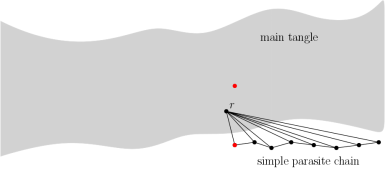
\includegraphics[width=3.0in]{figures/screenshot018.png}
%	\caption{simple sidechain attack [16], a series of deceptive sidechains will refer to a transaction r in the main network, when the SPC grows to a certain extent, it may lead to double success, the two in the figure A red dot represents a double flower transaction}
%	\label{simulationfigure}
%\end{figure}

%\begin{figure}[H]
%	\centering
%	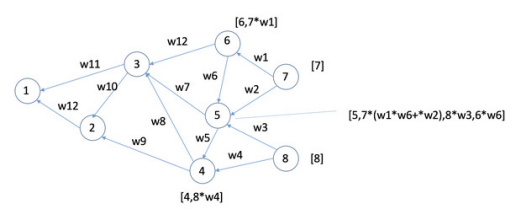
\includegraphics[width=3.0in]{figures/screenshot019.png}
%	\caption{Example of trading weights with side information}
%	\label{simulationfigure}
%\end{figure}

    %\begin{algorithm}[H]
	%\caption{Algorithm for calculating cumulative weight}
	%\KwIn{G^{'}=(V^{'} , E^{'})}
	%\KwOut{Cumulative weight}
	%graph traversal (BFS $\mid$ DFS) \Rightarrow  F(s) \; \\
	%V \gets F(s)\; \\
	%G(V,E) \Rightarrow G[F(s)]\,\,(\,let\,G(V,E)\,be\,the\,induced\,subgraph\,G[F(s)])\;   \\
	%Initialize\,F(v) \Leftarrow \left\{ \right\} for\,all\,v\in V\; \\
	%SortedVertices \Leftarrow topological\,sorting\,of\,G\; \\
	%\ForAll {$v$ such that $v\in SortedVertices$}{   
	%	\For{$i=v$ to $u$}{   
	%		\ $F(u) \Leftarrow $ F(u) + (F(v) + \left\{v\right\}) \ast w \; 
	%		}
	%	CumulativeWeight[v] \Leftarrow \left|F(v)\right| \; \\
	%	(Optimization)\,Free\,the\,memory\,taken,by\,F(v), as\,it\,no\,longer\,used
	%}	
	%\end{algorithm}

\subsection{Weight update algorithm based on flow graph calculation}
When updating the weight, the static graph algorithm needs to calculate the weight of each node from the beginning of the initial recognition node. The complexity of this algorithm is , if our static calculation information is cached, when the new tip is added. By updating the already cached information, the complexity of calculating the weight each time the tip is added can be differentiated . But there is also a problem with this, the spatial complexity of this algorithm will become . How to design a streaming algorithm to reduce the complexity of time space complexity to  is a challenge.

\begin{figure}[H]
	\centering
	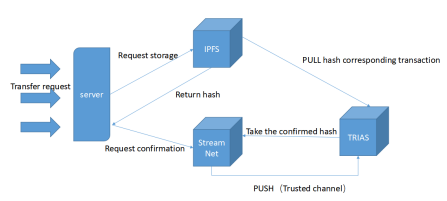
\includegraphics[width=3.0in]{figures/screenshot020.png}
	\caption{StreamNet shows the TRIAS transfer request cache}
	\label{simulationfigure}
\end{figure}

\subsection{Using StreamNet in conjunction with IPFS to cache TRIAS transfer requests}
StreamNet can be used to cache and pre-confirm other low-traffic blockchain systems because of its high throughput. TRIAS as a cross-blockchain system can take advantage of this feature to achieve its high degree of expansion, which can achieve the ability of elastic The specific structure is shown in Figure 20. There is a distributed transfer service. When an external transfer request comes over, it first stores the information transferred from the IPFS and gets a hash. The transfer server then constructs a hashNet transaction. When the traffic is small, StreamNet can directly push the hash of the transaction to TRIAS after confirming the transaction hash, so TRIAS can get the specific transfer information from IPFS and package the transfer. When the traffic is large, StreamNet will continue to confirm These transactions. When TRIA is idle, it will pull the confirmed hash to StreamNet, and get the specific transfer information from IPFS and package the transfer.

